\documentclass[a4paper,final,12pt]{article}
\usepackage{csquotes}
\usepackage[T1]{fontenc}
\usepackage{times}
\usepackage[english,brazil]{babel}
\usepackage{amssymb,amsfonts}
\usepackage{layouts}
\usepackage[top=3cm,bottom=3cm,left=3cm,right=3cm]{geometry}
\usepackage{indentfirst}
\usepackage{url}
\baselineskip=18pt
\setlength{\parskip}{6pt}
\setlength{\parindent}{24pt}
\usepackage{graphicx}
\usepackage{titlesec}
\usepackage{float}
\usepackage{biblatex}
\usepackage{soul}
\addbibresource{bibliografia.bib}


\title{Programação Concorrente \\ Implementação de um controlador de elevadores com \textit{threads}}
\author{Oseias Romeiro Magalhães / 211036123 \\ Prof. Eduardo Adilio Pelinson Alcheri}
\date{Junho de 2023}

\begin{document}

\maketitle

\begin{abstract}
Neste trabalho de Programação Concorrente, foi desenvolvido um controlador para lidar com as chamadas em cada andar de um prédio. Baseando-se no problema clássico do produtor-consumidor abordado em sala de aula \cite{pc}.
\end{abstract}

\section{Introdução}\label{section:introduction}
Um controlador de elevadores será abordado neste relatório como um exemplo prático de concorrência entre processos com memória compartilhada. O controlador deve receber chamadas vindo de vários andares e "desenhar" o melhor trajeto para o elevador seguir, no qual foi utilizado o algoritmo SCAN para esta tarefa. Mais detalhes será abordado na seção (\ref{section:description}) de descrição.

\section{Ambiente}\label{section:environment}

Para o desenvolvimento desse projeto, foi utilizado a linguagem C em ambiente Linux e compilado com GCC na versão 12.2. Utilizando as bibliotecas \textit{POSIX Pthreads} para utilização de estruturas de concorrências.

\section{Formalização do problema}\label{section:formalization}
O problema aborda o cenário onde vários usuários precisam se locomover por andares de um prédio de forma rápida. Para isso, existe um ou mais elevadores para atender as requisições em uma determinada quantidade de andares. Cada requisição é única, ou seja, só pode existir uma requisição por andar. Quando já existir uma requisição para todos os andares, qualquer outra requisição deve esperar até poder fazer sua chamada. Os elevadores também ficam em espera, caso não haja requisições para serem atendidas. Para lidar com o melhor trajeto que o elevador deva seguir, existe um decisor que decide o trajeto por meio de algum algoritmo de \textit{scheduler}.

\section{Descrição}\label{section:description}
O problema foi dividido em 3 (três) funções principais: \textit{elevator}, \textit{callsHandler} e \textit{decider}. Onde cada um é responsável por uma parte importante da implementação, contendo saídas de texto no terminal para acompanhar o processo.

\begin{figure}[h!]
  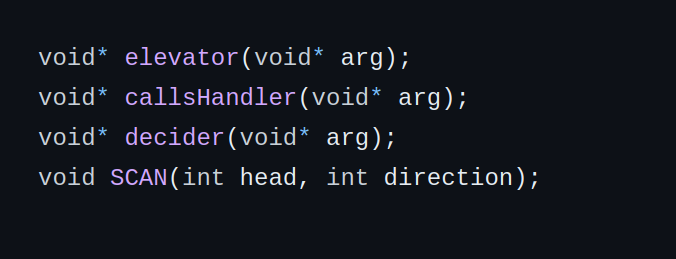
\includegraphics[scale=0.5]{imgs/functions.png}
  \caption{Funções}
  \label{fig:functions}
\end{figure}

Foi utilizado dois bufferes: \textit{callBuffer} e \textit{trackBuffer}, implementando assim dois cenários de produtor-consumidor utilizando \textit{mutex} e e variáveis de condições \cite{book}. Ambos bufferes são incicializados na \textbf{main} com o número de andares (valor impossível).

Além disso, existe as seguintes declarativas que configuram o cenário do problema:

\begin{figure}[h!]
  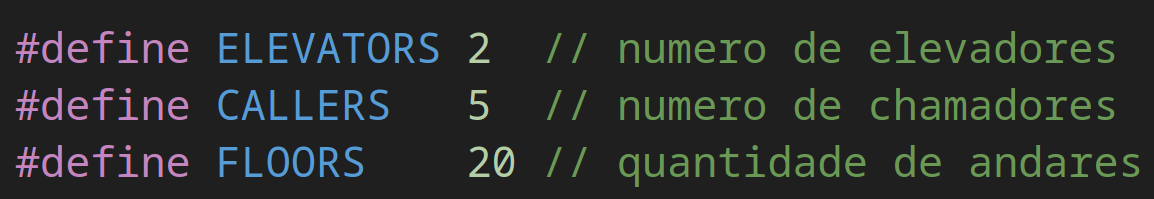
\includegraphics[scale=0.3]{imgs/declaratives.png}
  \caption{Declarativas}
  \label{fig:declaratives}
\end{figure}


\subsection{Controle de chamadas}\label{subsection:callsHandler}
A função \textit{callsHandler} é responsável por geração de chamadas forma randômica, garantindo também que cada chamada seja única, ou seja, não tenha mais de uma chamada por andar. Respaldo no cenário de que o elevador vai atender o andar independente da quantidade de usuários lá esperando, caso haja um número que exceda a quantidade permitida, os usuário devem se dividir. De qualquer forma, este cenário não é o foco do problema e nem é abordado pelo programa (também não sei por que o citei).

Cada chamada é gerada em uma thread e colocado em \textit{callBuffer}. Quando o buffer chegar no limite, as threads entram em espera. Como mencionado, as chamadas são únicas, logo o \textit{callBuffer} é limitado por NUM\_FLOORS (Figura \ref{fig:declaratives}). Caso, seja a primeira a adicionar uma chamada no buffer, então acorda o decisor (\ref{subsection:decider}), que deve estar esperando por novas chamadas.

\subsection{Elevadores}\label{subsection:elevators}
A função \textit{elevators} é responsável por consumir a chamadas em \textit{trackBuffer}, ou seja, atender as solicitações que o decisor (\ref{subsection:decider}) o passou, sendo consumido como uma fila. As regras no tocante ao limite do buffer e a lógica de concorrência é semelhante ao \textit{callBuffer} explicado na seção anterior.

\subsection{Decisor}\label{subsection:decider} 
O decisor tem como principal função, consumir as chamadas em \textit{callBuffer}, calcular a melhor rota para as chamadas até o momento e repassar para o \textit{trackBuffer} que será consumido pelos elevadores. Para traçar a melhor rota que o elevador deve assumir, foi utilizado o algoritmo de SCAN \cite{scan} que considera a posição do elevador e o sentido, subindo ou descendo. O sentido é alternado a cada vez que o decisor executa e quanto a posição, é considerado a do primeiro elevador. O decisor, fica em estado de espera quando o o buffer está vazio, e libera o \textit{mutex} de chamada assim que a rota é calculada.

\subsection{SCAN}\label{subsection:scan}
O algoritmo usado no decisor (\ref{subsection:decider}) para "desenhar" a melhor rota é o SCAN. Algoritmo de escalonamento que consegue encontrar uma rota com menor custo de deslocamento e tempo ocioso dos passageiros, com base na posição do elevador e o sentido de prioridade (descida/subida), ordenando e dividindo as chamadas em duas sub listas (andares abaixo e acima da posição do elevador), criando um trajeto para percorrer as duas sub listas da melhor forma. O algoritmo foi traduzido para C e adaptado para a o problema, com uso dos bufferes que são variáveis globais, sendo assim, acessível pela função SCAN (Figura \ref{fig:functions}).

\pagebreak

\begin{figure}[h!]
  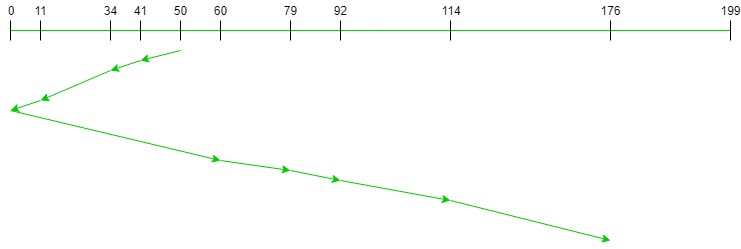
\includegraphics[scale=0.5]{imgs/scan.jpg}
  \caption{SCAN}
  \label{fig:scan}
\end{figure}

\section{Fluxo de execução}\label{result}
Assim que executado o programa, os elevadores e o decisor entrará em espera enquanto é feita as chamadas, então o decisor é acordado, realizando as operações necessárias e assim, liberando os chamadores e acordando os elevadores. O que é mostrado na tela do terminal por meios de \textit{prints}. A quantidade de  elevadores, andares e usuaraios que fazem a chamada podem ser editados pelas declarativas mostradas na Figura \ref{fig:declaratives}.


\section{Conclusão}
Portanto, foi desenvolvido assim, um programa que aborda um problema prático envolvendo comunicação entre processos através de memória compartilhada. Assim como requisitado para o trabalho final da disciplina.

\printbibliography

\end{document}
